\documentclass[tikz,border=2pt]{standalone}
\usepackage{amsmath}
\usepackage{pgfplots}
\pgfplotsset{compat=1.18}

\begin{document}
% Left: the point (cos x, sin x) on the unit circle after rotating (1,0) by the angle x.
% Right: the graphs of sin and cos over one period 2π, and tan with its asymptotes.
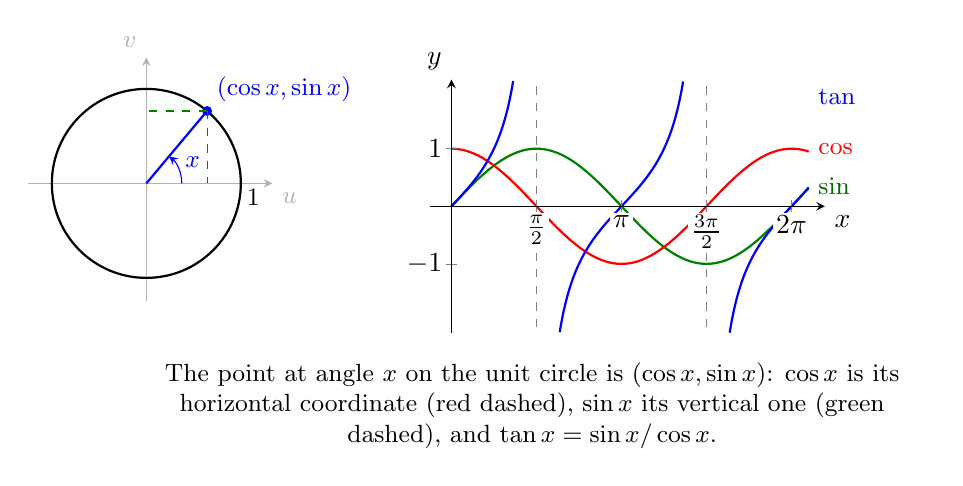
\begin{tikzpicture}
	\begin{scope}
		\draw[gray!60, -stealth] (-1.5,0) -- (1.6,0) node[below right, font=\small] {$u$};
		\draw[gray!60, -stealth] (0,-1.5) -- (0,1.6) node[above left, font=\small] {$v$};
		\draw[thick] (0,0) circle (1.2);
		\draw[thick, blue] (0,0) -- (50:1.2);
		\fill[blue] (50:1.2) circle (1.8pt);
		\draw[red, dashed] (50:1.2) -- ({1.2*cos(50)},0);
		\draw[green!50!black, dashed] (50:1.2) -- (0,{1.2*sin(50)});
		\draw[blue, -stealth] (0.45,0) arc (0:50:0.45);
		\node[blue, font=\small] at (25:0.65) {$x$};
		\node[blue, above right, font=\small] at (50:1.2) {$(\cos x,\sin x)$};
		\node[below right, font=\small, inner sep=2pt] at (1.2,0) {$1$};
	\end{scope}
	\begin{axis}[
		at={(3.6cm,-1.9cm)}, anchor=south west,
		axis lines=middle,
		xmin=-0.4, xmax=6.9,
		ymin=-2.2, ymax=2.2,
		xtick={1.5708,3.1416,4.7124,6.2832}, xticklabels={$\tfrac\pi2$,$\pi$,$\tfrac{3\pi}2$,$2\pi$},
		ytick={-1,1}, tick label style={fill=white, inner sep=1pt}, axis on top,
		xlabel={$x$}, ylabel={$y$},
		xlabel style={below right}, ylabel style={above left},
		samples=200, smooth, clip=false,
		width=6.6cm, height=4.8cm
		]
		\addplot[thick, green!50!black, domain=0:6.6] {sin(deg(x))};
		\addplot[thick, red, domain=0:6.6] {cos(deg(x))};
		\addplot[thick, blue, domain=0:1.14, samples=60] {tan(deg(x))};
		\addplot[thick, blue, domain=2.0:4.28, samples=80] {tan(deg(x))};
		\addplot[thick, blue, domain=5.14:6.6, samples=60] {tan(deg(x))};
		\draw[gray, dashed] (axis cs:1.5708,-2.1) -- (axis cs:1.5708,2.1);
		\draw[gray, dashed] (axis cs:4.7124,-2.1) -- (axis cs:4.7124,2.1);
		\node[green!40!black, anchor=west, font=\small] at (axis cs:6.6,0.35) {$\sin$};
		\node[red, anchor=west, font=\small] at (axis cs:6.6,1.0) {$\cos$};
		\node[blue, anchor=west, font=\small] at (axis cs:6.6,1.9) {$\tan$};
	\end{axis}
	\node[anchor=north, align=flush center, text width=10cm, font=\small] at (4.9,-2.15) {The point at angle $x$ on the unit circle is $(\cos x,\sin x)$: $\cos x$ is its horizontal coordinate (red dashed), $\sin x$ its vertical one (green dashed), and $\tan x=\sin x/\cos x$.};
\end{tikzpicture}
\end{document}
